% -----------------------------------------------------------------------------
% Engineering chapter section for the Formula Student acceleration vehicle.
% Designed for inclusion in latex/CombinedFinal/main_single_file.tex.
% Requires the master file to load: styling.sty, biblatex, tabularx, siunitx,
% graphicx, subcaption, float and the references_wheel_assembly.bib file.
% -----------------------------------------------------------------------------
\providecommand{\figbox}[2]{\begin{figure}[H]\centering\fbox{\parbox[c][#1][c]{0.92\linewidth}{\centering #2}}\caption{#2}\end{figure}}

\chapterauthor{Wheel Assembly Design}{Ziyang Xing}
\vspace{-25px}
%\contribution{This chapter presents the author's individual engineering contribution to the Formula Student acceleration vehicle: the wheel assembly, suspension, steering and braking design, with detailed focus on the rear multi-link suspension, anti-squat/toe strategy, and single inboard brake acting on the limited-slip differential.}
\label{chap:wheel_assembly_design}

\section{Wheel assembly design scope and key terminology}

\subsection{Scope of this chapter}
This chapter presents the wheel-assembly design for the acceleration-only Formula Student UK vehicle. The previous chapter establishes the vehicle-level event objective; this chapter explains how the suspension, steering and braking choices support that objective at the wheel-assembly level. The front suspension, steering system and front brakes are included because they are required for a complete and rule-compliant vehicle, but the main engineering contribution is the rear wheel assembly. The rear design combines multi-link kinematics, a tunable anti-squat target, dynamic rear toe control, and a single inboard brake acting on the limited-slip differential (LSD).

The vehicle is not intended to be a balanced skidpad, autocross and endurance car. Its useful dynamic case is launch and short straight-line acceleration. The rear suspension can therefore be biased towards rear traction, ride-height control, low scrub and wheel-end mass reduction. The chosen wheel package is the OZ Racing Formula Student Hybrid Carbon CL \SI{10}{in} wheel and Hoosier 18.0 x 6.0-10 Formula Student slick tyre. OZ lists the 7 x 10 in hybrid carbon wheel at approximately \SI{1.35}{kg}, while Hoosier lists the 18.0 x 6.0-10 slick at approximately \SI{9}{lb} \parencite{zxOZCarbon10,zxHoosierSpecs}. These light components make the remaining upright, brake and link mass important to the corner-mass budget.

\subsection{Definitions used in the design argument}
\textit{Toe angle} is the plan-view angle between the wheel and the vehicle centreline. \textit{Toe-in} points the front of the wheel inwards; \textit{toe-out} points it outwards. Small rear toe-in can improve straight-line stability, while zero toe reduces tyre scrub and power loss in straight running \parencite{zxSuspensionSecretsToe}. \textit{Camber} is the front-view wheel inclination relative to vertical. It is secondary for this acceleration-only design, but it must remain adjustable to compensate for manufacturing and setup variation.

\textit{Squat} is the rear suspension compression caused by acceleration load transfer. \textit{Anti-squat} is a geometric force-path effect that resists this compression. The driven tyre force passes through the suspension links; if the side-view force line is inclined, a vertical jacking component is generated. Anti-squat is therefore part of the same suspension-kinematics problem as bump steer, wheel-centre path and compliance steer \parencite{zxMilliken1995,zxDixon2009}. \textit{Bump steer} is toe change during wheel bump or rebound. \textit{Unsprung mass} is mass that moves with the wheel, including wheel, tyre, hub, upright and outboard brake hardware.

%\figbox{26mm}{Terminology schematic placeholder: plan-view toe, front-view camber, side-view squat/anti-squat force path, and inboard versus outboard brake location.}
\begin{figure}[H]
\centering
\begin{subfigure}[t]{0.49\linewidth}
    \centering
    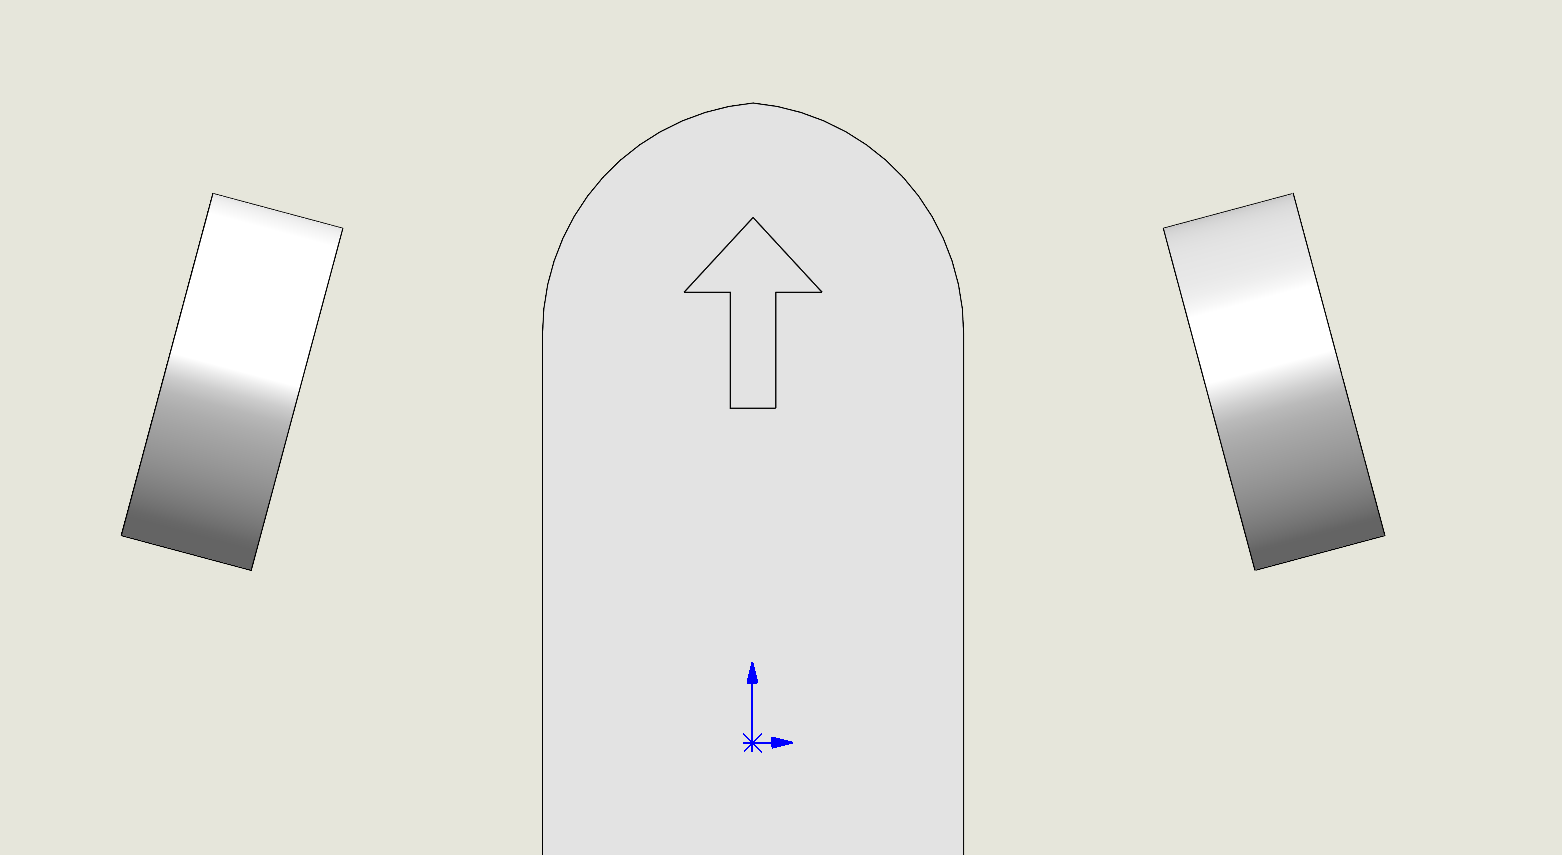
\includegraphics[width=\linewidth]{figures/Toe_Demo.png}
    \caption{Top view visual of a car with toe in.}
\end{subfigure}\hfill
\begin{subfigure}[t]{0.49\linewidth}
    \centering
    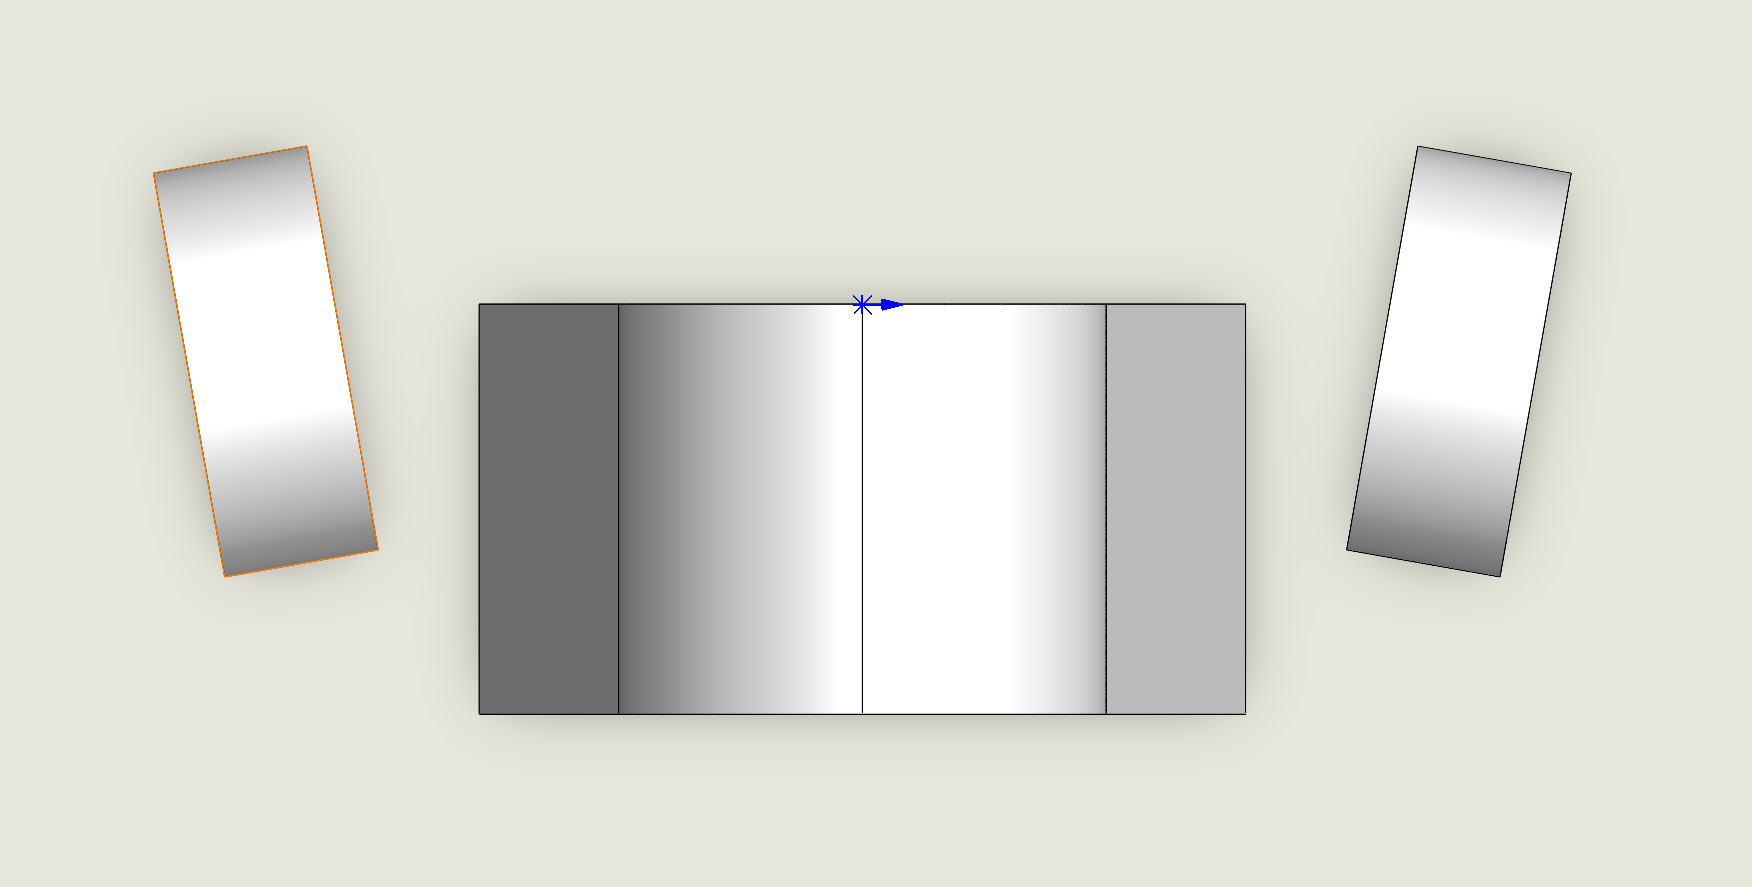
\includegraphics[width=\linewidth]{figures/Camber_Demo.png}
    \caption{Front view visual of a car with negative camber.}
\end{subfigure}
\caption{Visualizations for the suspension terminology.}
\label{fig:susp_terms_defines}
\end{figure}
\subsection{Wheel-assembly requirements}
The wheel assembly requirements were derived from rear traction, mass reduction, adjustability, rule compliance and subsystem integration. Table~\ref{tab:reqs_wheel} gives a concise flow-down from requirement area to design evidence. The table is intentionally compact: detailed vehicle-level acceleration targets are treated in the vehicle dynamics chapter, while this chapter concentrates on the physical wheel-assembly implications.

\begin{table}[H]
\centering
\caption{Wheel-assembly requirements used to guide the design.}
\label{tab:reqs_wheel}
\setlength{\tabcolsep}{4pt}
\begin{tabularx}{\linewidth}{|>{\raggedright\arraybackslash}p{0.24\linewidth}|>{\raggedright\arraybackslash}X|>{\raggedright\arraybackslash}X|}
\hline
\textbf{Requirement area} & \textbf{Design implication} & \textbf{Evidence in chapter} \\
\hline
Rear traction and stability & Resist launch squat and control rear toe & Multi-link layout; 100\% anti-squat target; dynamic toe strategy \\
\hline
Low wheel-end mass & Remove rear outboard brake hardware where rules allow & Single inboard brake acting on the LSD \\
\hline
Setup adjustability & Treat anti-squat and toe values as tunable starting points & Upright-side shim/spacer strategy \\
\hline
Rule compliance & Keep steering and braking mechanical, inspectable and conservative & Rack-based steering; hydraulic braking; LSD brake rule discussion \\
\hline
System integration & Avoid suspension geometry that conflicts with drivetrain or chassis & Shared rear bay package and interface checks \\
\hline
\end{tabularx}
\end{table}

Table~\ref{tab:materials_wheel} gives the representative component and material choices used in the design calculations. These choices are conservative rather than exotic: the steering and front brake hardware are kept familiar for inspection, while the rear suspension and brake package carry the main originality.

\begin{table}[H]
\centering
\caption{Representative component and material choices used in the wheel assembly design.}
\label{tab:materials_wheel}
\setlength{\tabcolsep}{4pt}
\begin{tabularx}{\linewidth}{|>{\raggedright\arraybackslash}p{0.23\linewidth}|>{\raggedright\arraybackslash}p{0.29\linewidth}|>{\raggedright\arraybackslash}X|}
\hline
\textbf{Component} & \textbf{Selected part/material} & \textbf{Reason for selection} \\
\hline
Wheel & OZ Racing Formula Student Hybrid Carbon CL 10 in & Low mass and Formula Student-specific wheel package \\
\hline
Tyre & Hoosier 18.0 x 6.0-10 slick & Compact 10 in tyre suitable for the selected wheel envelope \\
\hline
Suspension links & 4130 chromoly steel tube, nominally \SI{12.7}{mm} OD and \SI{1.2}{mm} wall & High stiffness and strength in compact tension/compression members; final tube size checked by link-force analysis \parencite{zxMatweb4130} \\
\hline
Uprights & 7075-T6 aluminium billet & High-strength machinable material for compact pickup geometry \parencite{zxMatweb7075} \\
\hline
Brake calipers & Wilwood GP200 & Lightweight compact two-piston caliper for tight packaging; Wilwood lists GP200 at approximately 0.90 lb / less than 1 lb \parencite{zxWilwoodGP200} \\
\hline
Shim/spacer packs & Machined aluminium or steel spacers & Repeatable setup adjustment at the upright-side pickups \\
\hline
\end{tabularx}
\end{table}

\section{Concept selection for wheel assembly architecture}

Concept selection used Pugh matrices to compare layouts against mass, unsprung mass, launch traction, kinematic control, adjustability, manufacturability, packaging and inspection risk. The rear suspension options were double wishbone, semi-trailing/trailing arm, beam-like rear structure and multi-link. A multi-link layout was selected because it gives the greatest freedom to tune anti-squat and toe independently. This agrees with the general multi-link design principle that separate link locations allow greater geometric flexibility than a conventional wishbone arrangement; Altair also notes that rear multi-link suspensions are commonly described as five-link systems \parencite{zxAltairMultilink}.

\begin{table}[H]
\centering
\caption{Pugh matrix for rear suspension concept selection.}
\label{tab:pugh_susp_wheel}
\setlength{\tabcolsep}{3pt}
\begin{tabularx}{\linewidth}{|>{\raggedright\arraybackslash}X|c|c|c|c|}
\hline
\textbf{Criterion} & \textbf{Double wishbone} & \textbf{Semi-trailing} & \textbf{Beam/rigid} & \textbf{Multi-link} \\
\hline
Longitudinal traction support & 0 & 0 & 0 & + \\
\hline
Toe-control potential & 0 & - & -- & ++ \\
\hline
Anti-squat tuning freedom & + & 0 & - & ++ \\
\hline
Packaging with LSD brake & 0 & + & 0 & + \\
\hline
Mass/manufacturability & 0 & + & ++ & - \\
\hline
Setup adjustability & + & 0 & - & ++ \\
\hline
Inspection risk & + & 0 & + & 0 \\
\hline
Indicative result & Medium & Medium & Low/medium & Highest \\
\hline
\end{tabularx}
\end{table}

The rear brake concepts were conventional outboard rear brakes, two inboard rear brakes, a single inboard LSD brake and a motor-side brake. Formula Student UK requires hydraulic braking on all four wheels, two independent circuits and protection from drivetrain failure, but Rule T6.1.3 states that a single brake acting on a limited-slip differential is acceptable \parencite{zxFSUK2026Rules}. The single inboard LSD brake was selected because it gives the clearest unsprung-mass reduction while retaining a rule-supported mechanical braking path. A Wilwood GP200 billet aluminium caliper was selected as the representative caliper because Wilwood lists it as a compact unit of less than \SI{1}{lb} and notes its suitability for limited-space applications \parencite{zxWilwoodGP200}.

\begin{table}[H]
\centering
\caption{Pugh matrix for rear brake/drivetrain layout selection.}
\label{tab:pugh_brake_wheel}
\setlength{\tabcolsep}{3pt}
\begin{tabularx}{\linewidth}{|>{\raggedright\arraybackslash}X|c|c|c|c|}
\hline
\textbf{Criterion} & \textbf{Outboard rear} & \textbf{Dual inboard} & \textbf{Single LSD brake} & \textbf{Motor-side} \\
\hline
Rule alignment & + & + & + & 0 \\
\hline
Unsprung-mass reduction & -- & + & ++ & ++ \\
\hline
Total mass & - & 0 & + & 0 \\
\hline
Upright packaging & - & + & ++ & ++ \\
\hline
Failure-mode clarity & + & 0 & 0 & - \\
\hline
Inspection/service access & + & 0 & + & - \\
\hline
Indicative result & Medium & Medium & Highest & Medium/risky \\
\hline
\end{tabularx}
\end{table}

Steering was kept conventional because it is not the main performance differentiator. A rack-based system with direct mechanical actuation, rack-mounted stops and visible mechanical joints was selected. This follows the Formula Student steering requirements for mechanical actuation, rack stops and limited steering free play \parencite{zxFSUK2026Rules,zxFSG2026Rules}.

The driven-wheel architecture was selected using the same Pugh-matrix method as the suspension and braking concepts. A quad-motor all-wheel-drive layout offers the greatest theoretical control authority, but its benefit is reduced for this acceleration-only vehicle because the centre of gravity is deliberately placed rearward. Under peak launch acceleration, the car is close to the wheelie or tipping limit, so the front axle is lightly loaded and front-wheel drive contributes less useful tractive force than it would in a more balanced vehicle. The additional motors, inverters, shafts, cooling requirements and control software would therefore add substantial mass, cost and complexity for a limited performance gain. A single-motor rear-wheel-drive layout was selected as the most appropriate architecture because it is lighter, cheaper, simpler to integrate and more compatible with the limited-slip differential and single inboard brake package.

\begin{table}[H]
\centering
\caption{Pugh matrix for driven-wheel architecture selection.}
\label{tab:pugh_drive_architecture}
\setlength{\tabcolsep}{3pt}
\begin{tabularx}{\linewidth}{|>{\raggedright\arraybackslash}X|c|c|c|}
\hline
\textbf{Criterion} & \textbf{AWD quad motor} & \textbf{Dual-motor RWD} & \textbf{Single-motor RWD} \\
\hline
Peak acceleration potential & + & + & 0 \\
\hline
Usefulness with rearward centre of gravity & - & + & ++ \\
\hline
Front-axle traction benefit near wheelie limit & - & 0 & + \\
\hline
Total vehicle mass & -- & - & ++ \\
\hline
Powertrain cost & -- & - & ++ \\
\hline
Mechanical and electrical complexity & -- & - & ++ \\
\hline
Packaging around wheel assemblies & -- & - & ++ \\
\hline
Control calibration risk & -- & - & ++ \\
\hline
Reliability and serviceability & - & 0 & + \\
\hline
Compatibility with LSD and inboard brake package & -- & - & ++ \\
\hline
Indicative result & Performance gain, high penalty & Medium & Highest \\
\hline
\end{tabularx}
\end{table}

The single-motor rear-wheel-drive option was therefore selected. This choice does not maximise theoretical traction in isolation, but it gives the best system-level compromise for an acceleration-only design. The rearward mass distribution already biases normal load towards the driven axle during launch, while the vehicle's proximity to the wheelie limit reduces the practical value of adding front drive. The selected architecture also reduces integration risk and leaves more packaging freedom for the rear multi-link suspension, limited-slip differential and inboard brake assembly.

\section{Rear wheel assembly design}

\subsection{Rear multi-link geometry and nomenclature}
The rear assembly is shown in Figure~\ref{fig:rear_views_wheel}. In the top view, the front of the vehicle is towards the bottom of the image. The most aft separate member is the toe link; the forward separate member is the pushrod. The fore and aft upper and lower links are compact and nearly overlap in some views.

\begin{figure}[H]
\centering
\begin{subfigure}[t]{0.49\linewidth}
    \centering
    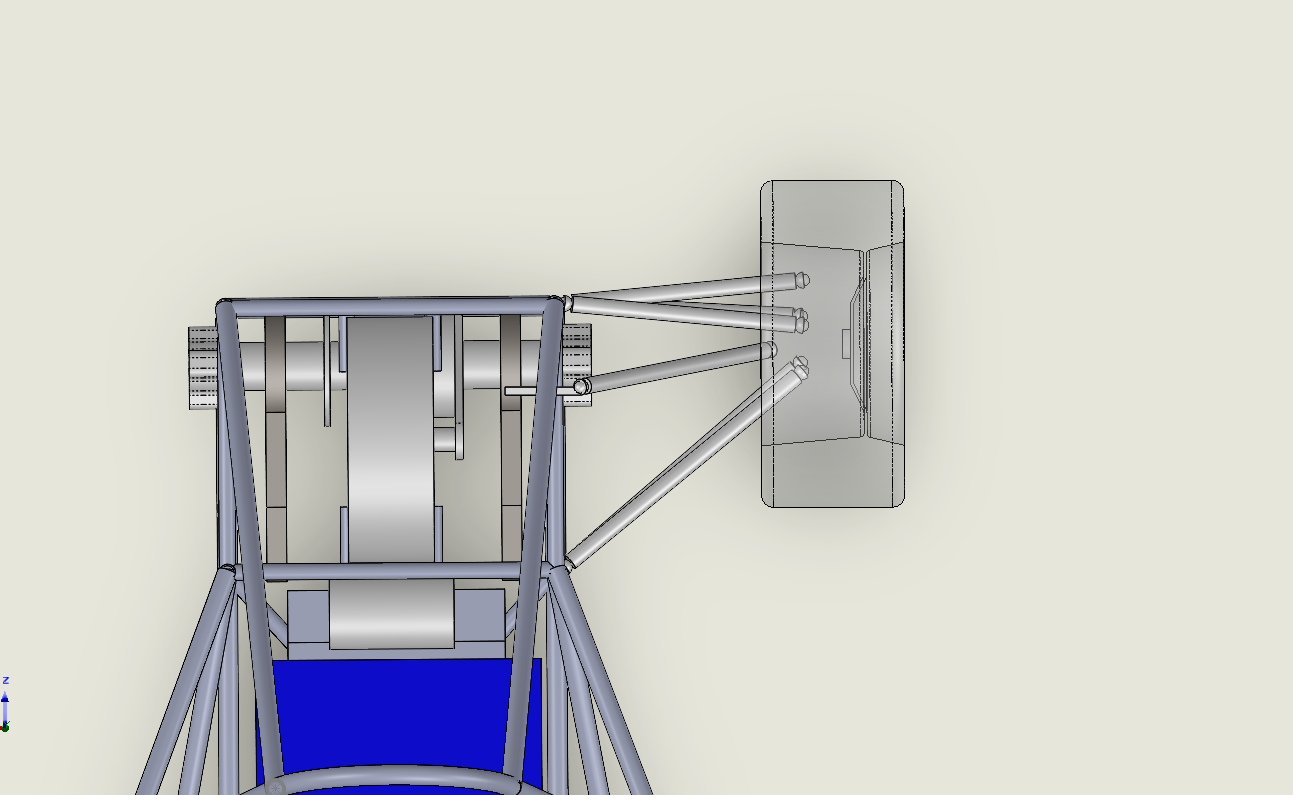
\includegraphics[width=\linewidth]{figures/rear_top_view.png}
    \caption{Top view.}
\end{subfigure}\hfill
\begin{subfigure}[t]{0.49\linewidth}
    \centering
    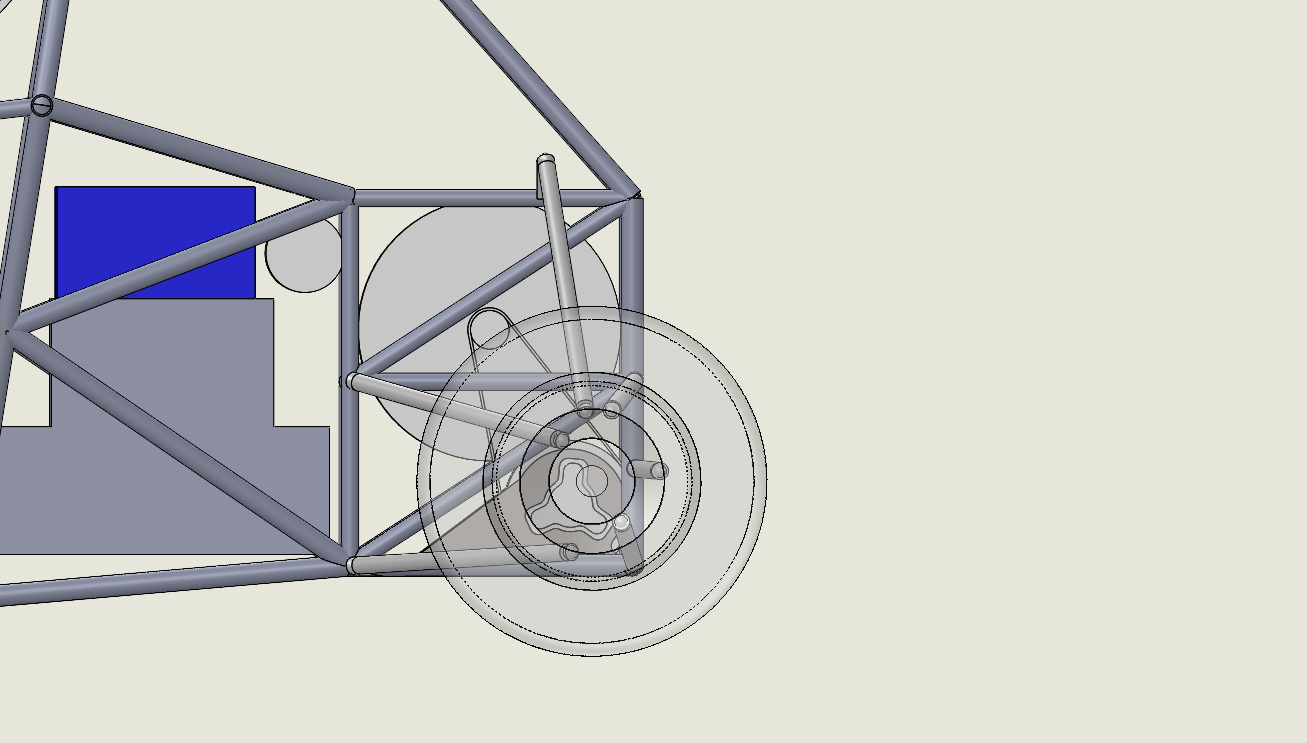
\includegraphics[width=\linewidth]{figures/rear_side_view.png}
    \caption{Side view.}
\end{subfigure}
\caption{CAD views of the rear multi-link wheel assembly. The top view identifies the rear-mounted toe link and the forward pushrod; the side view shows the shallow locating links and steep pushrod.}
\label{fig:rear_views_wheel}
\end{figure}

The suspension is described as a rear multi-link layout with five wheel-locating links plus a pushrod. The wheel-locating links are the fore/aft upper links, fore/aft lower links and rear-mounted toe link. The pushrod transfers wheel motion to the spring-damper actuation path and is not counted as a primary wheel-locating link. The chassis-side hardpoints are intentionally simple and approximately rectangular. The kinematic design work is concentrated at the upright side, where ball-joint pickup positions define anti-squat, toe-link angle and bump-steer response.

This packaging choice also improves design clarity. A welded chassis-side pickup is expensive to move once the frame is built, whereas an upright-side bracket can include machined spacers, alternative shim packs and measured setup positions. The design therefore separates structural simplicity from kinematic adjustability. The rear frame provides the load path and protects the drivetrain bay; the upright bracket design provides the final setup freedom. This is particularly valuable because the chosen toe and anti-squat values are intended as starting points for testing, not as unchangeable answers.

\subsection{Upright-side hardpoints and setup adjustability}
The 100\% anti-squat and \SI{0.15}{\degree} static rear toe-in values are educated starting values rather than fixed final settings. Formula Student setup work must account for measurement uncertainty, hardpoint tolerance, tyre behaviour and test feedback; quick adjustment of toe, camber and ride-height related variables is therefore good practice \parencite{zxOptimumGtips}.

The upright-side joint centres are implemented using brackets with shim or spacer packs. Vertical shims at the upright-side control-link pickups change the side-view link angles and therefore the anti-squat percentage. Vertical adjustment at the toe-link pickup changes the toe-link angle through wheel travel and tunes bump steer. Lateral shims set static camber and toe. Fore-aft shimming is not used because it is less repeatable under suspension load. Link lengths are set initially and then fixed, so trackside setup is mainly performed with shim packs.

\begin{table}[H]
\centering
\caption{Planned upright-side adjustment strategy.}
\label{tab:shim_strategy_wheel}
\setlength{\tabcolsep}{4pt}
\begin{tabularx}{\linewidth}{|>{\raggedright\arraybackslash}p{0.30\linewidth}|>{\raggedright\arraybackslash}X|>{\raggedright\arraybackslash}X|}
\hline
\textbf{Adjustment feature} & \textbf{Primary effect} & \textbf{Use in testing} \\
\hline
Vertical control-link shims & Side-view link angle and instant-centre position & Anti-squat tuning around the 100\% starting target \\
\hline
Vertical toe-link pickup adjustment & Toe-link angle relative to wheel travel & Bump-steer / toe-curve tuning \\
\hline
Lateral shim packs & Lateral joint-centre position & Static camber and toe correction \\
\hline
Toe-link length & Nominal toe during build & Initial setup, then fixed \\
\hline
\end{tabularx}
\end{table}

\begin{figure}[H]
\centering
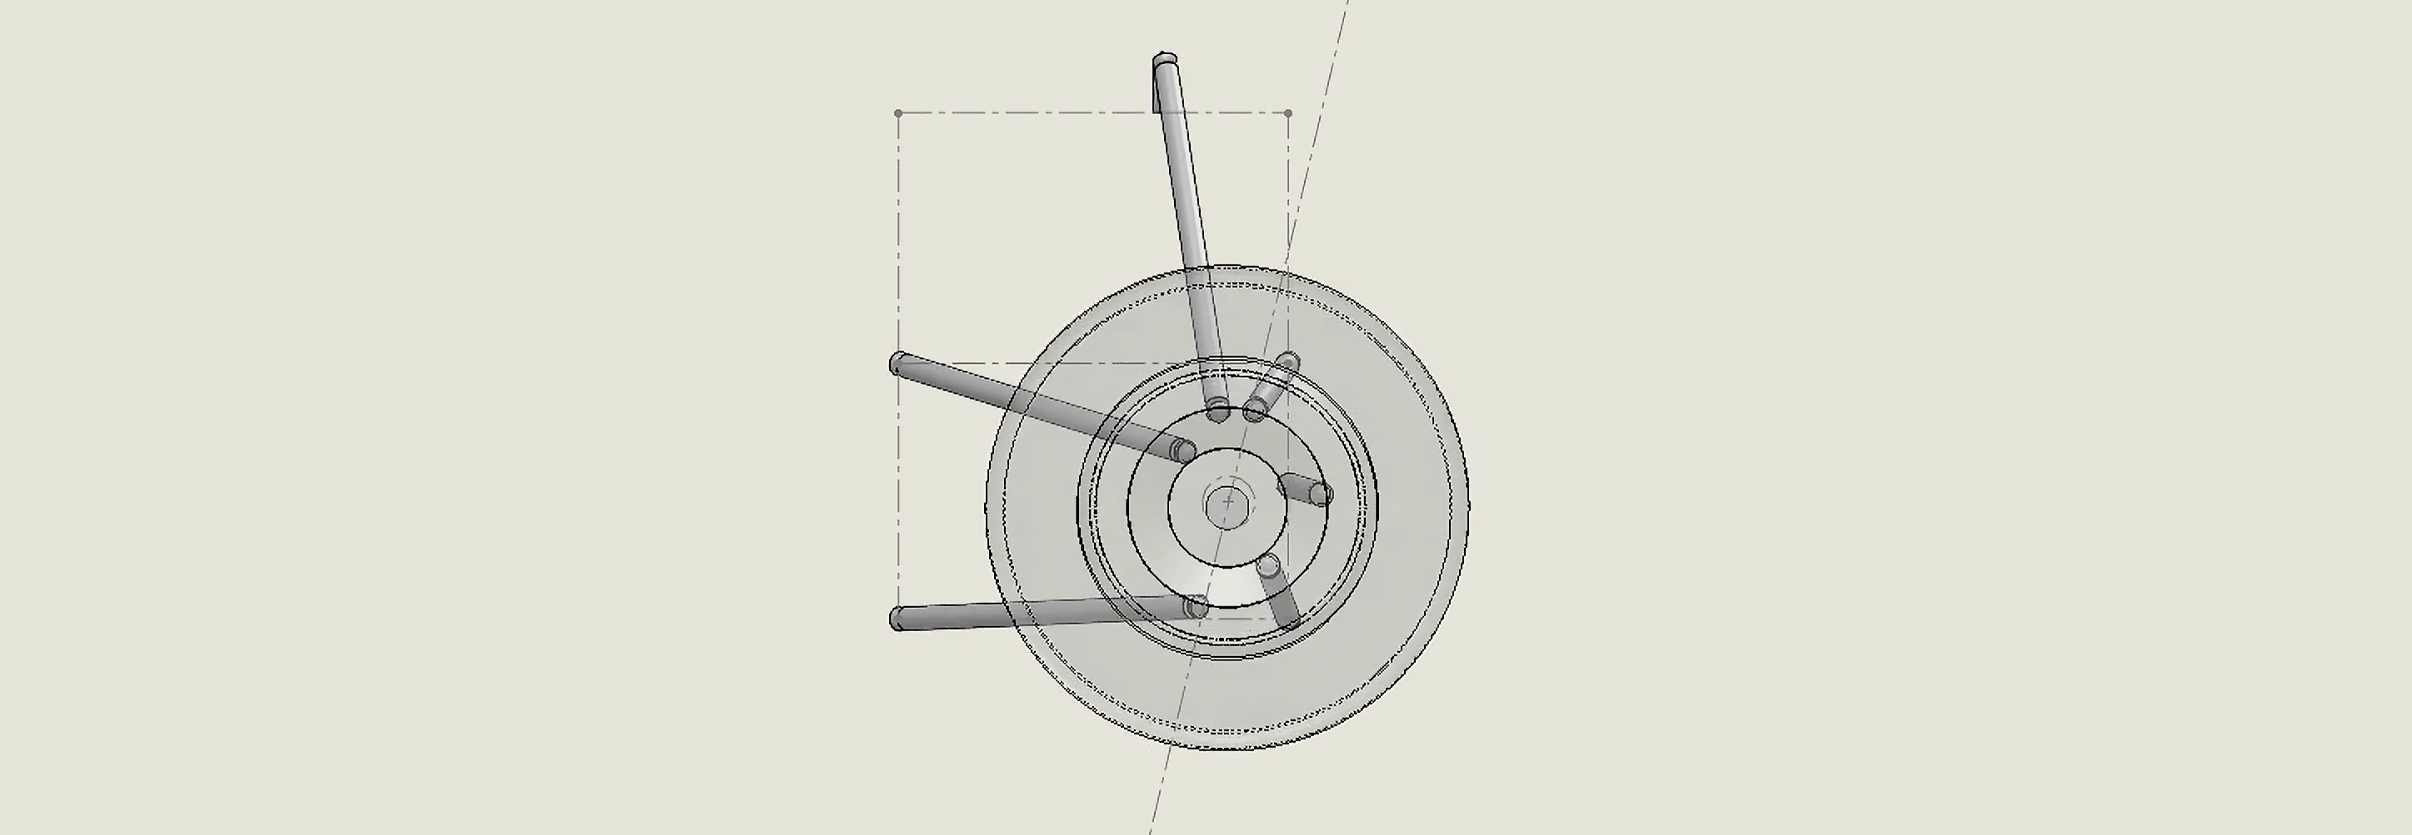
\includegraphics[width=0.78\linewidth]{figures/rear_susp_motion.png}
\caption{Rear suspension motion view used to check that the toe link, pushrod and wheel-locating links remain separated and inspectable through the expected travel range.}
\label{fig:rear_motion_wheel}
\end{figure}

\subsection{Preliminary link angles and force basis}
Screenshot-derived side-view measurements show shallow locating-link angles of approximately X to \SI{12}{\degree} relative to horizontal and a much steeper pushrod angle of approximately X to \SI{80}{\degree}. The final CAD hardpoint table records the exact upper, lower and toe-link angles as X\(^{\circ}\), X\(^{\circ}\) and X\(^{\circ}\). The force-analysis design basis is \SI{230}{kg} vehicle mass and \SI{1.3}{g} maximum acceleration:
\begin{equation}
F_{x,\mathrm{total}} = ma = 230 \times 1.3 \times 9.81 \approx \SI{2.93}{kN}.
\end{equation}
If the two driven rear wheels share the load equally, \(F_{x,\mathrm{wheel}} \approx \SI{1.47}{kN}\). With the nominal anti-squat line angle of \SI{12.7}{\degree}, the idealised vertical jacking component is
\begin{equation}
F_{z,\mathrm{AS}} \approx F_{x,\mathrm{wheel}}\tan(12.7^\circ)
\approx \SI{0.33}{kN}
\end{equation}
per rear wheel.

For a representative side-view link angle of \(\alpha=\SI{10}{\degree}\), the axial force associated with the anti-squat component is
\begin{equation}
N_{\mathrm{AS,link}}\approx\frac{F_{z,\mathrm{AS}}}{2\sin\alpha}
=\frac{0.33}{2\sin10^\circ}\approx\SI{0.95}{kN}.
\end{equation}
The longitudinal contribution is
\begin{equation}
N_{x,\mathrm{link}}\approx\frac{F_{x,\mathrm{wheel}}}{2\cos\alpha}
=\frac{1.47}{2\cos10^\circ}\approx\SI{0.75}{kN}.
\end{equation}
The indicative link force is therefore about \(\sqrt{0.95^2+0.75^2}\approx\SI{1.2}{kN}\) before safety factors and transient loads. The wheel-locating links are selected as 4130 chromoly steel tube, nominally \SI{12.7}{mm} outside diameter and \SI{1.2}{mm} wall thickness, with threaded inserts and rod ends. Uprights are machined from 7075-T6 aluminium, with steel or aluminium shim packs and 4130 steel chassis brackets where welded load paths are needed.

\subsection{Anti-squat and dynamic toe-control strategy}
Anti-squat geometry limits rear suspension compression during acceleration \parencite{zxSuspensionSecretsAntiSquat}. The initial target is 100\% anti-squat, corresponding to a \SI{12.7}{\degree} side-view force line. This value is a rational reference point for an acceleration-only car because the design objective is launch stability and rear geometry control, not all-round handling. It is not treated as a proven optimum; if testing shows excessive jacking or wheel hop, vertical shims at the upright-side pickups reduce the effective anti-squat.

The static rear toe target is \SI{0.15}{\degree} toe-in. This gives initial straight-line stability, while the dynamic target is approximately zero rear toe at speed to reduce scrub. The contact-patch force at speed is
\begin{equation}
F_{x,\mathrm{rear}}\approx ma+D+F_{rr},
\end{equation}
so the anti-squat geometry responds not only to the force accelerating the vehicle, but also to the force required to overcome drag and rolling resistance. Drag also acts above ground level. Assuming the effective centre of pressure is higher than the centre of mass, the rear load-transfer contribution can be estimated as
\begin{equation}
\Delta N_{\mathrm{rear}}\approx\frac{ma h_{\mathrm{CG}}+D z_D}{L}.
\end{equation}
With the final aerodynamic model, \(D=X\,\mathrm{N}\) at X km/h and \(z_D=X\,\mathrm{m}\). This gives X N additional rear load transfer and a rear jacking displacement of X mm. Reading from the toe curve, the rear toe at X km/h is X\(^{\circ}\), satisfying the target of approximately zero toe at speed.

\figbox{30mm}{Rear toe curve placeholder: rear toe angle against wheel displacement or vehicle speed, showing \SI{0.15}{\degree} static toe-in and approximately zero toe at X km/h.}

\subsection{Single inboard brake acting on the LSD}
The rear brake acts on the LSD. This is the clearest rule-facing description because the Formula Student UK rules explicitly allow a single brake acting on a limited-slip differential \parencite{zxFSUK2026Rules}. The layout removes rear wheel-end brake discs and calipers, reducing rear unsprung mass and simplifying the upright package. The estimated saving is \SI{3.6}{kg} of rear unsprung mass and \SI{0.9}{kg} total mass relative to a conventional outboard rear brake arrangement.

\begin{table}[H]
\centering
\caption{Rear brake bill-of-materials comparison.}
\label{tab:bom_mass_wheel}
\setlength{\tabcolsep}{4pt}
\begin{tabularx}{\linewidth}{|>{\raggedright\arraybackslash}X|>{\raggedright\arraybackslash}p{0.22\linewidth}|>{\raggedright\arraybackslash}p{0.20\linewidth}|>{\raggedright\arraybackslash}X|}
\hline
\textbf{Layout} & \textbf{Rear unsprung mass effect} & \textbf{Total mass effect} & \textbf{Implication} \\
\hline
Two outboard rear brakes & Baseline & Baseline & Conventional but heavier wheel-end package \\
\hline
Single inboard brake acting on LSD & \(-\SI{3.6}{kg}\) & \(-\SI{0.9}{kg}\) & Lower rear corner mass and freer upright packaging \\
\hline
\end{tabularx}
\end{table}

The final brake package uses a Wilwood GP200 caliper, an X mm steel disc and an aluminium caliper mount tied into the rear frame bay. Brake design remains safety-critical: hydraulic pressure, piston area, effective radius, pedal force, brake balance and thermal capacity must be checked according to normal brake-design practice \parencite{zxLimpert2011}. The Formula Student rules also require protection from drivetrain failure and moving parts \parencite{zxFSUK2026Rules}.

\begin{figure}[H]
\centering
\begin{subfigure}[t]{0.49\linewidth}
    \centering
    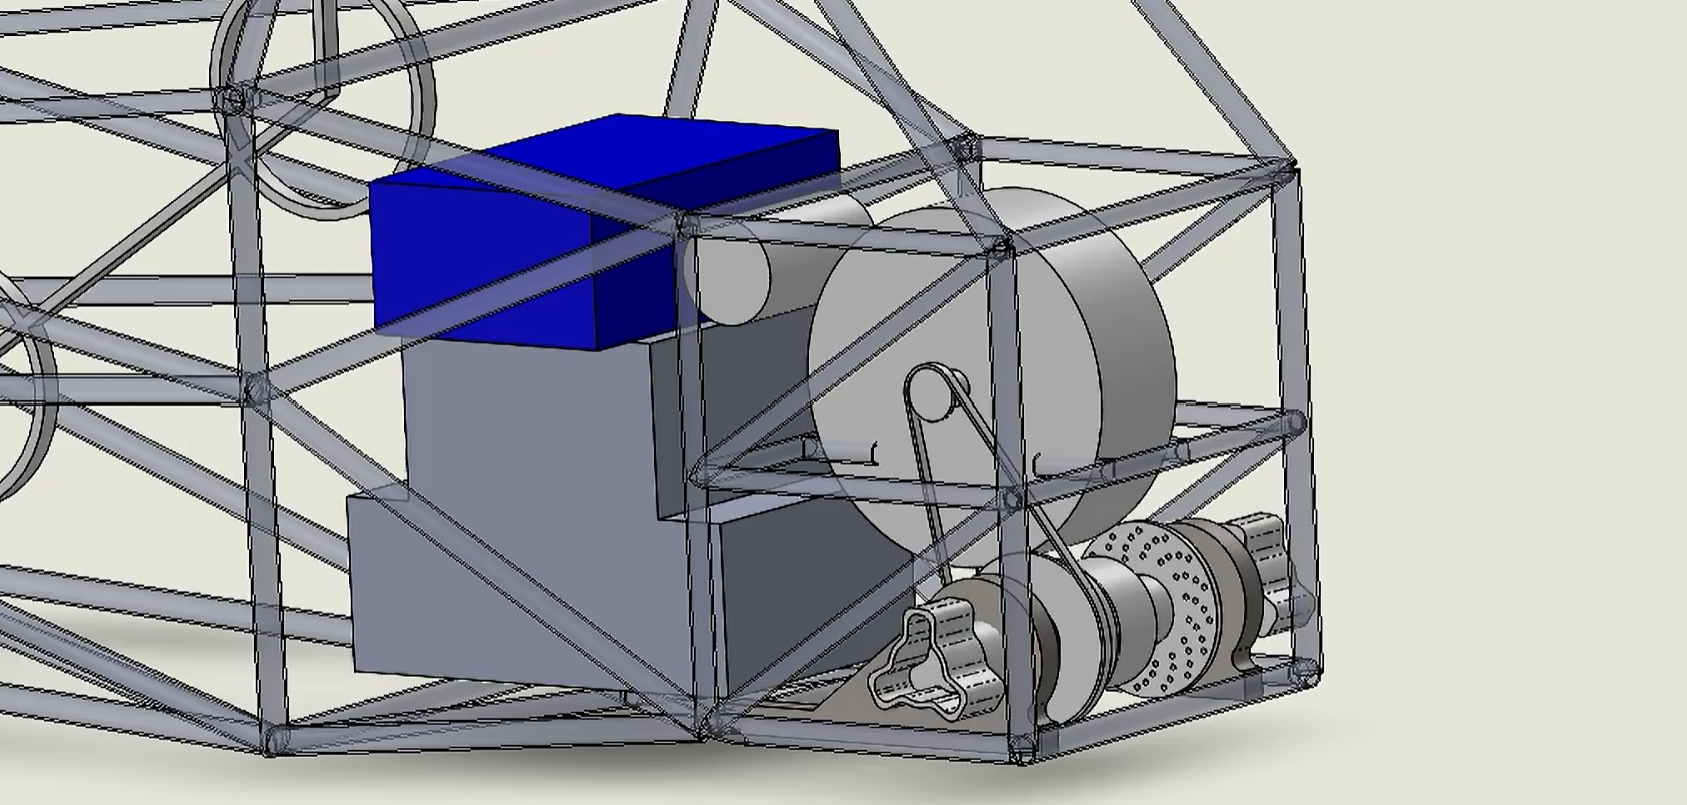
\includegraphics[width=\linewidth]{figures/powertrain_view.png}
    \caption{Central drivetrain bay for the LSD brake concept.}
\end{subfigure}\hfill
\begin{subfigure}[t]{0.49\linewidth}
    \centering
    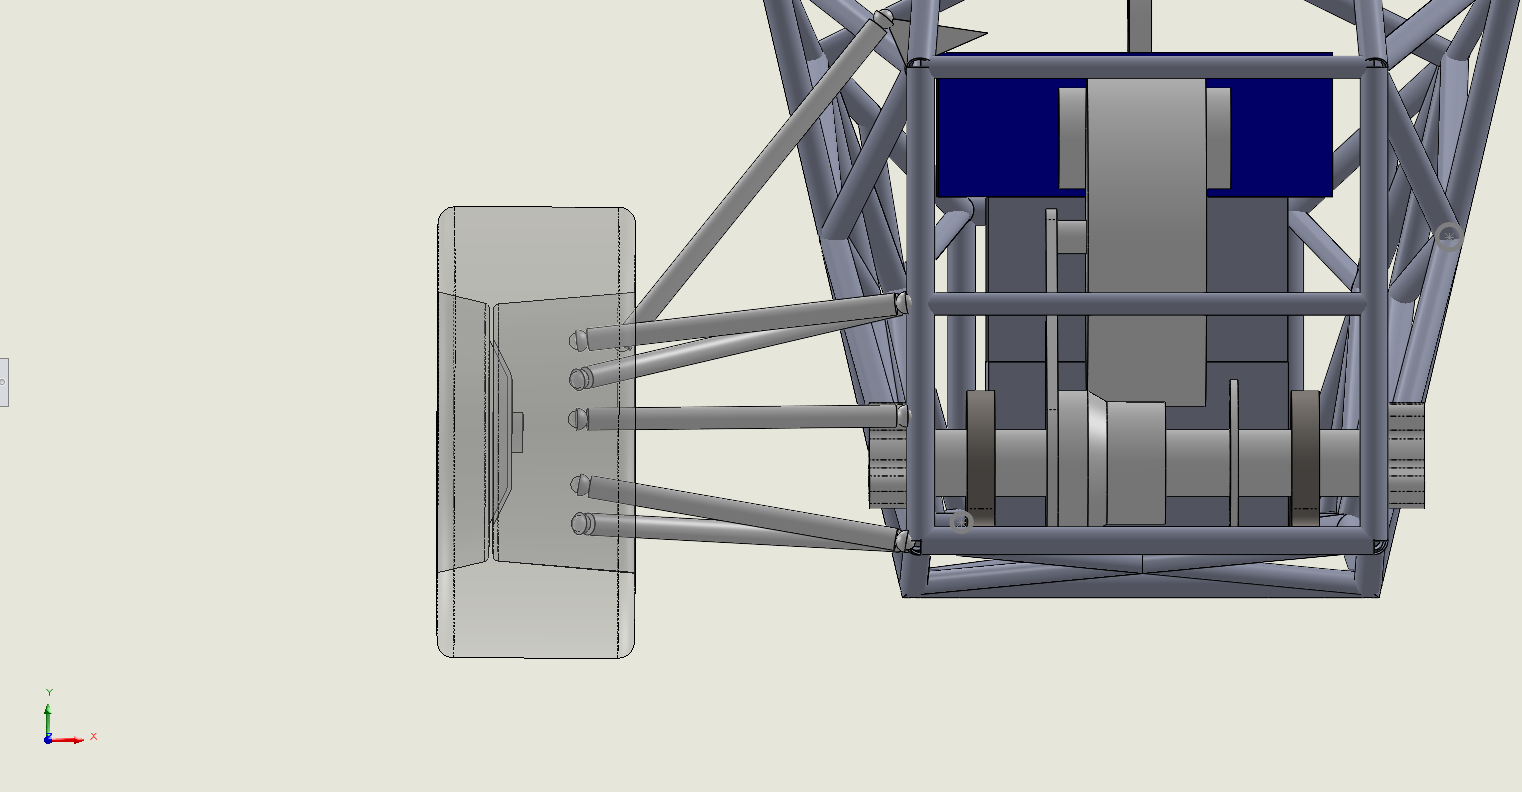
\includegraphics[width=\linewidth]{figures/rear_inboard_view.png}
    \caption{In-car rear view of the LSD/final-drive region.}
\end{subfigure}
\caption{Rear powertrain and brake integration region.}
\label{fig:rear_powertrain_package_wheel}
\end{figure}

\subsection{Rear assembly risks and mitigations}
The rear design integrates wheel location, spring-damper actuation, toe control, anti-squat tuning, drivetrain output and braking. The main risks are hardpoint sensitivity, excessive anti-squat, incorrect toe-at-speed behaviour and brake/drivetrain integration. These are mitigated through shim-adjustable upright-side pickups, load-based link sizing, a tunable toe-link pickup and a protected inboard brake package. The rear assembly is therefore not a fixed one-shot geometry; it is a tunable acceleration-focused axle concept.

\begin{table}[H]
\centering
\caption{Rear assembly risks and design mitigations.}
\label{tab:rear_risks_wheel}
\setlength{\tabcolsep}{4pt}
\begin{tabularx}{\linewidth}{|>{\raggedright\arraybackslash}p{0.25\linewidth}|>{\raggedright\arraybackslash}X|>{\raggedright\arraybackslash}X|}
\hline
\textbf{Risk} & \textbf{Effect on vehicle} & \textbf{Mitigation in design} \\
\hline
Hardpoint sensitivity & Toe curve or anti-squat differs from design intent & Upright-side shim packs and CAD coordinate checks \\
\hline
Excessive jacking & Wheel hop or harsh launch response & 100\% anti-squat treated as adjustable starting target \\
\hline
Incorrect toe-at-speed response & Too much scrub or unstable toe-out & Rear toe link, vertical pickup adjustment and lateral shim setting \\
\hline
Brake/drivetrain interaction & Concentrated central brake torque and protection requirement & Brake acts on LSD; guard, torque and failure-mode checks included \\
\hline
\end{tabularx}
\end{table}

\section{Front wheel assembly, steering and braking design}

The front wheel assembly is deliberately conventional. The front suspension is a compact double-wishbone arrangement using 4130 steel links, 7075-T6 aluminium uprights and rod-end joints with misalignment spacers. Its role is to locate the front wheels, maintain straight-line tracking and support steering and braking. Static camber is X\(^{\circ}\), front toe is X\(^{\circ}\), and the bump-steer target is less than X\(^{\circ}\) over the expected front wheel travel.

The steering system uses a compact rack-and-pinion layout with a continuous-perimeter steering wheel, quick-release hub, steering column, compact rack, tie rods and steering arms. A direct column is used where packaging allows; one high-quality universal joint is used if the final column angle requires it. The rack is mechanically attached to the primary structure, and steering stops act on the rack. This low-risk choice reflects the Formula Student steering requirements and keeps the main novelty in the rear assembly \parencite{zxFSUK2026Rules,zxFSG2026Rules}.

The front brakes provide the main inspection confidence and braking capacity. They use small outboard discs, Wilwood GP200 calipers and a conventional hydraulic circuit. The rear LSD brake reduces rear wheel-end mass, but the overall brake system still uses two independent hydraulic circuits as required by the rules \parencite{zxFSUK2026Rules}. The final brake-balance calculation gives X\% front bias and X\% rear bias at a pedal force of X N.

\begin{table}[H]
\centering
\caption{Front steering and braking elements retained for low-risk compliance.}
\label{tab:front_elements_wheel}
\setlength{\tabcolsep}{4pt}
\begin{tabularx}{\linewidth}{|>{\raggedright\arraybackslash}p{0.27\linewidth}|>{\raggedright\arraybackslash}p{0.28\linewidth}|>{\raggedright\arraybackslash}X|}
\hline
\textbf{Element} & \textbf{Design choice} & \textbf{Reason} \\
\hline
Steering gear & Compact rack-and-pinion & Direct mechanical steering with rack-mounted stops \\
\hline
Column route & Direct column or one U-joint & Low free play and visible mechanical joints \\
\hline
Front brakes & Outboard discs and GP200 calipers & Conservative inspection and braking capacity \\
\hline
Front links & 4130 steel double-wishbone links & Simple load paths and reliable fabrication \\
\hline
\end{tabularx}
\end{table}

%\figbox{30mm}{Front suspension, steering and brake drawing placeholder: double-wishbone links, upright, steering arm, rack/tie rods and front brake package.}
\begin{figure}[H]
\centering
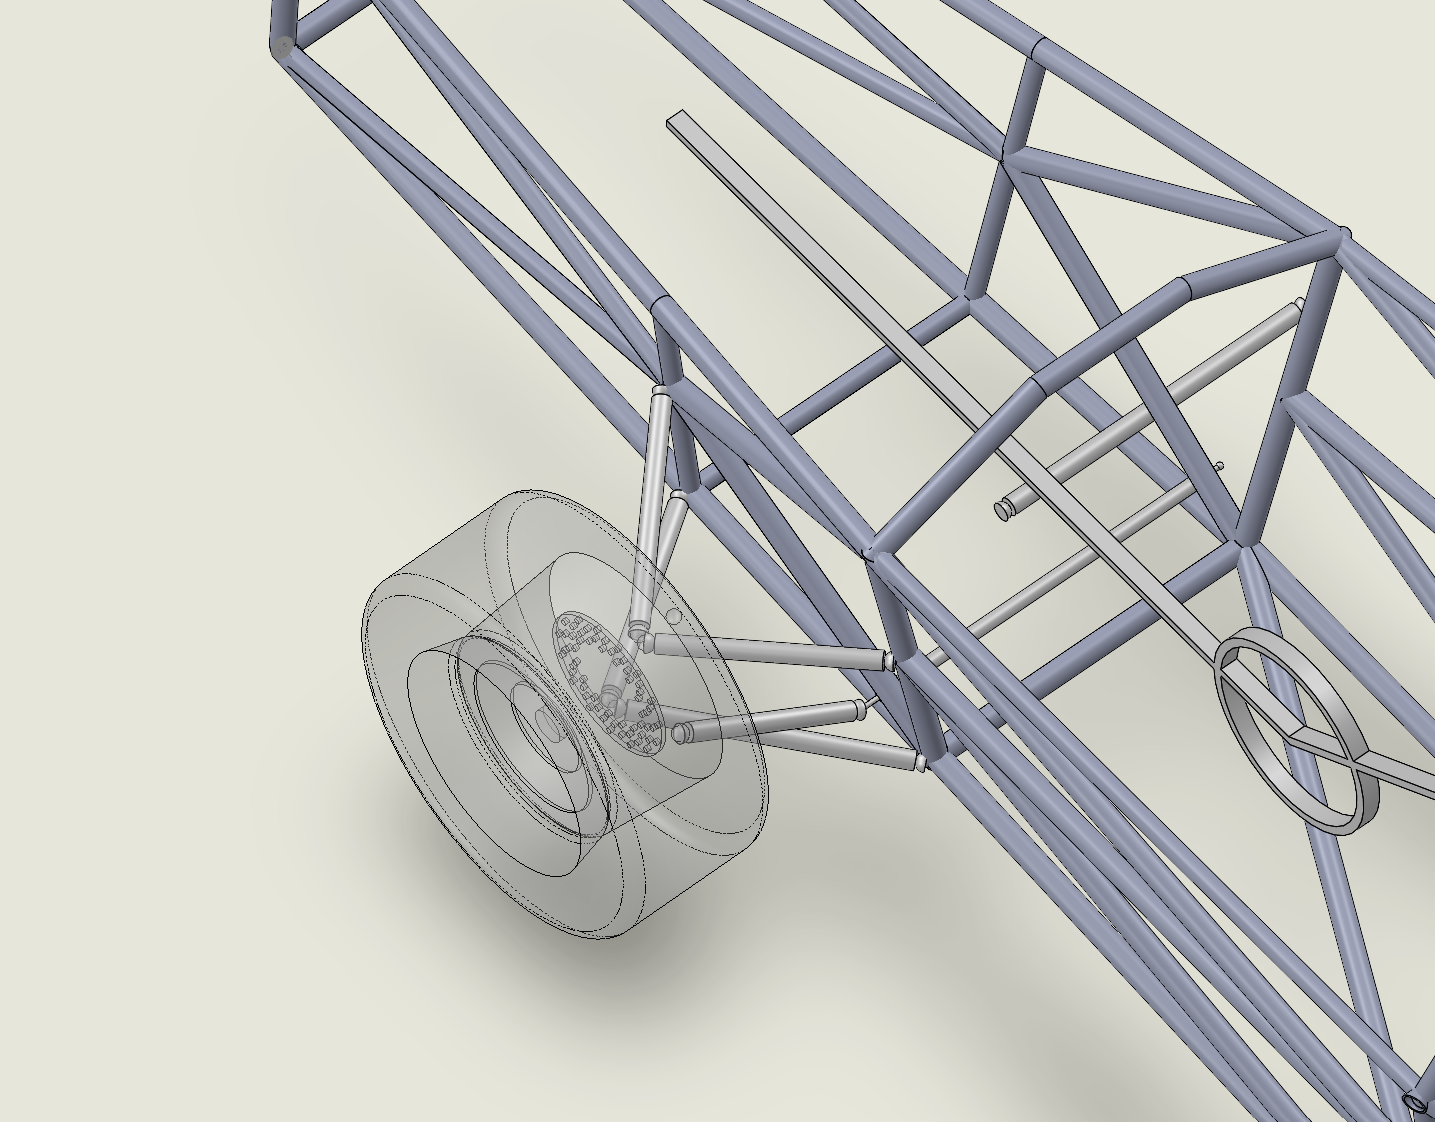
\includegraphics[width=0.78\linewidth]{figures/Front_Preview.png}
\caption{Preview of the front suspension and strring rack layout.}
\label{fig:front_preview}
\end{figure}

\section{System integration and teamwork}

The rear suspension was developed with the chassis, drivetrain, braking and vehicle-dynamics work rather than as an isolated mechanism. The simple rectangular chassis-side hardpoint arrangement gives manufacturable load paths and reduces the risk that late setup changes require chassis redesign. The upright-side shim system then provides the tuning freedom.

The powertrain and rear suspension occupy the same rear bay. The LSD, final drive, chain, brake disc, caliper, links and pushrod must all maintain clearance. The brake acts on the LSD, so its mount and guarding are part of the drivetrain package as well as the braking package. The vehicle-dynamics interface provides the \SI{230}{kg}, \SI{1.3}{g} load case, centre-of-mass height X m, centre-of-pressure height X m and drag at X km/h.

\begin{table}[H]
\centering
\caption{Subsystem interfaces used to keep the wheel assembly consistent with the vehicle.}
\label{tab:interfaces_wheel}
\setlength{\tabcolsep}{4pt}
\begin{tabularx}{\linewidth}{|>{\raggedright\arraybackslash}p{0.22\linewidth}|>{\raggedright\arraybackslash}X|>{\raggedright\arraybackslash}X|}
\hline
\textbf{Interface} & \textbf{Information exchanged} & \textbf{Design response} \\
\hline
Chassis & Hardpoint envelope and bracket load paths & Rectangular chassis-side pickups retained \\
\hline
Drivetrain & LSD, final drive and chain line & Brake and rear links packaged around central drivetrain bay \\
\hline
Vehicle dynamics & Mass, acceleration, drag and toe targets & Anti-squat and toe strategy tuned for acceleration run \\
\hline
Braking & Caliper/disc package and hydraulic layout & Single LSD brake integrated with front hydraulic circuit \\
\hline
Steering & Rack and tie-rod geometry & Conventional front steering retained for low risk \\
\hline
\end{tabularx}
\end{table}

Shared CAD reviews, mass-budget updates and rule checks were used to control these interfaces. This is important because the rear axle is not only a suspension design; it is a combined suspension, brake and drivetrain module. The design therefore satisfies the engineering requirement that individual work remains connected to the wider group design rather than optimising one isolated component.
\iffalse
\section{Evidence, limitations and final verification}

The design evidence consists of Pugh matrices, CAD packaging, component selection, preliminary anti-squat geometry, link-force calculations, the rear brake mass comparison and subsystem interface checks. The final verification values are: anti-squat line angle X\(^{\circ}\), anti-squat percentage X\%, static rear toe X\(^{\circ}\), toe at X km/h equal to X\(^{\circ}\), rear jacking displacement X mm, front bump-steer range X\(^{\circ}\), front brake torque X Nm, rear LSD brake torque X Nm and maximum suspension-link axial force X kN with a factor of safety of X.

\begin{table}[H]
\centering
\caption{Final design evidence to be reported from CAD and calculation outputs.}
\label{tab:evidence_wheel}
\setlength{\tabcolsep}{4pt}
\begin{tabularx}{\linewidth}{|>{\raggedright\arraybackslash}p{0.30\linewidth}|>{\raggedright\arraybackslash}X|>{\raggedright\arraybackslash}X|}
\hline
\textbf{Evidence item} & \textbf{Reported value} & \textbf{Design purpose} \\
\hline
Anti-squat construction & 12.7\(^{\circ}\), X\% after final CAD check & Confirms launch geometry target \\
\hline
Toe curve & 0.15\(^{\circ}\) static, X\(^{\circ}\) at X km/h & Confirms low-scrub speed condition \\
\hline
Suspension link load & X kN maximum, factor of safety X & Sizes 4130 links and brackets \\
\hline
Brake torque & X Nm front, X Nm rear LSD & Confirms braking compliance and balance \\
\hline
Mass comparison & -3.6 kg unsprung, -0.9 kg total & Justifies inboard LSD brake \\
\hline
\end{tabularx}
\end{table}

The main limitation is specialisation. A 100\% anti-squat starting target increases sensitivity to hardpoint tolerance, bracket stiffness and compliance. This is acceptable for an acceleration-only vehicle but is not claimed as an all-round Formula Student optimum. The dynamic toe strategy depends on drag, centre-of-pressure height and measured toe curve; the assumption \(z_D>h_{\mathrm{CG}}\) must be checked against the aerodynamic model. The LSD brake layout saves mass but concentrates braking torque in the central drivetrain package, requiring guarding, torque capacity and inspection access.
\fi
\section{Conclusion}

This chapter has presented the wheel assembly, suspension, steering and braking design for the acceleration-only Formula Student UK vehicle. The front systems are intentionally conventional: they provide controllability, braking confidence and rule compliance. The main contribution is the rear wheel assembly, where multi-link kinematics, dynamic toe behaviour and inboard braking are integrated.

The rear suspension uses five wheel-locating links plus a pushrod. The chassis-side pickups are simple and rectangular, while the upright-side hardpoints and shim packs provide tuning. The 100\% anti-squat target, corresponding to a \SI{12.7}{\degree} side-view force line, is an educated starting point for launch control. The \SI{0.15}{\degree} static rear toe-in is likewise an initial setup value, intended to move towards approximately zero toe at speed as the anti-squat and drag-related load state changes.

The rear brake acts on the LSD and removes outboard rear brake hardware. The expected saving is \SI{3.6}{kg} unsprung mass and \SI{0.9}{kg} total mass. The result is not a generic suspension package, but an acceleration-event-specific rear axle concept: start from a rational rear-traction setup, make the geometry adjustable, and reduce wheel-end mass while retaining rule-compliant steering and braking systems.
